\documentclass{beamer}
%\usepackage{verbatime}
\usepackage{subfig}
\usepackage{palatino}
\usepackage[utf8]{inputenc}
\mode<presentation>
{
\title{IT Workshop Presentation}
\subtitle{Comparing Different Sorting Algorithms}
\author[Kanak, Siddharth]
{Kanak Singhal\inst{1} \and Siddharth Goyal\inst{2}}
 
\institute[LNMIIT] 
{
  \inst{1}%
  15UCS057\\
  LNMIIT
  \and
  \inst{2}%
  15UCS140\\
  LNMIIT
}
%\setbeamertemplate{items}[square]
%\setbeamertemplate{footline}[page number]
\usetheme{Copenhagen}
\usecolortheme{beaver}
%\setbeamertemplate{navigation symbols}{}
}
\begin{document}
%\tikzstyle{every picture}+=[remember picture]
\begin{frame}
\titlepage
\end{frame}

\begin{block}{GNU Plot of Number of comparisions vs Size of Array}
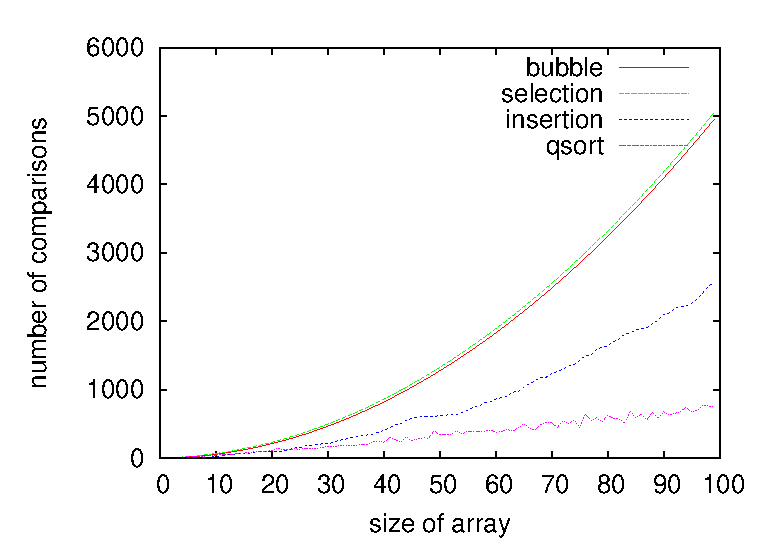
\includegraphics[scale=0.75]{noc.eps}
\end{block}

\begin{frame}
\begin{block}{GNU Plot of Time vs Size of Array}
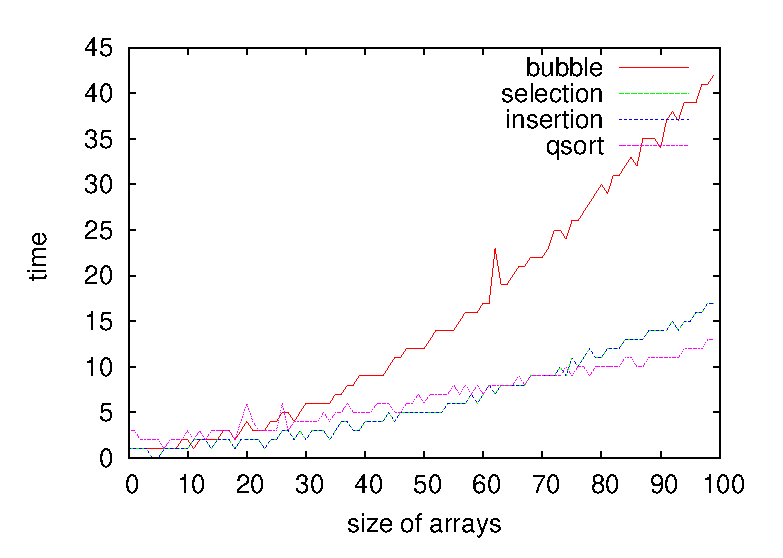
\includegraphics[scale=0.75]{time.eps}
\end{block}
\end{frame}

\begin{frame}
\frametitle{Conclusions}
\framesubtitle{From analyzing the above graphs:-}
\setlength{\unitlength}{1.8cm}
%\begin{figure}[H]
%\hspace{-5cm}
%\begin{centering}
%{
%\begin{picture}(1.8,1.8)
%\thicklines
%\put(0,0){\line(0,1){1}}
%\put(0,0){\line(1,0){1}}
%\put(0,1){\line(1,0){1}}
%\put(1,0){\line(0,1){1}}
%\end{picture}
%}
%\end{centering}
%\end{figure}
\begin{itemize}
\item The efficiency of different algorithms can be analyzed by taking into consideration the number of comparisions and the time taken by the algorithm to sort Vs the size of array
\item This model is independent of the hardware configuration of the machine.
\item The best alhgorithm among the analysis is the Quick Sort algorithm
\item The worst algorithm is the Selection algorithm.
\end{itemize}
\end{frame}

\end{document}
